\documentclass[10pt,conference,compsocconf]{IEEEtran}

\usepackage{hyperref}
\usepackage{graphicx}	% For figure environment
\usepackage{amsmath}
\usepackage{amssymb}
\usepackage{float}


\begin{document}
\title{CS-433 Machine Learning Project 1}

\author{
  Matthias Minder, Zora Oswald, Silvan Stettler\\
  
}

\maketitle

\begin{abstract}
%%% abstract here
\end{abstract}

\section*{Introduction}
Collision events in the Large Hadron Collider at CERN do not create directly observable results. An essential part of elementary particles such as the Higgs boson therefore rely on classifying the collisions based on a number of variables that can be measured in the collider. 
In our dataset, a vector containing 30 dimensions describes one collision event. A binary classification algorithm can be used to predict the presence of a Higgs boson based on this feature vector. The model is trained with data from collisions for which the existence of a Higgs boson is determined.
Our classifications of the collision events consist of three main steps:
\begin{enumerate}
\item Normalization and imputation of missing data 
\item Parameter optimization using cross-validation
\item Predictions on test data using the best-fitting binary model 
\end{enumerate}
Furthermore, the importance of variables for the final model was assessed using best subset selection.
\section*{Methods}
As a first step, all features were transformed to have mean zero and unit variance, disregarding missing values.
\par 
As a second step, missing values were imputed. These missing values are due to physical measures being made impossible under certain conditions. However, since the classification methods used in the scope of this project don't naturally support the presence of missing values, they were imputed using the following linear regression approach: 
\par
Analysis of the raw data showed that there are a total of six distinct patterns of missing features. A pattern of observation $\boldsymbol{x}$, denoted $P(\boldsymbol{x})$, is characterized by values of $\boldsymbol{x}$ missing in dimensions $M$ and values being present in dimensions $M'$. Approximately 60'000 observations of the training data contained no missing values, i.e. $M_{P(\boldsymbol{x})} = \emptyset$. For each incomplete pattern $P_i(\boldsymbol{x})$ and every missing feature $l \in M_{P_i(\boldsymbol{x})}$, a linear regression was fitted to complete observations, taking all features $k \in M'_{P_i(\boldsymbol{x})}$ as observations and feature $l$ as response. This fit was then applied to impute the missing feature $l$ of all $\boldsymbol{x}$ corresponding to $P_i(\boldsymbol{x})$. All linear regression models were fitted using gradient descent. Missing values of the test data were imputed using the fits on the training data.  
\par
This method for missing value imputation was chosen because it follows the natural structure of the data: Observations corresponding to the same physical preconditions leading to a specific pattern of missing values were all subjected to the same fit for missing value imputation. Simple linear regression was chosen due to its easy interpretability. Fitting more complex regression models would only make limited sense, since the absence of "true" values for a given missing value pattern makes reasonable model comparison impossible. Finally, we chose this approach over "simple", constant imputation using the feature mean or median because it allows to capture more of the data variability. 
\par
However, by imputing missing values, the information about their underlying physical reasons is lost. To capture this information, dummy variables were created that encode every non-complete pattern of missing values. 
%\begin{align*}
%{x}_{ij, j \in M} &\approx w_0 + \sum_{k \in M'} w_k {x}_{ik}\\
%\boldsymbol{w}^* = \underset{x}{argmin}\sum_i & ({x}_{ij, j \in M} - \boldsymbol{x}^T_{ik, k \in M'} \boldsymbol{w})^2\\
%{x}_{na,ij, j \in M} &= w_0 + \sum_{k \in M'} w_k {x}_{na,ik}
%\end{align*} 
\par
% I finge da chönnt me no e besseri übrleitig mache, so im sinn vo aus nächsts heimer s fittet odr so
Classifying the collision events comes down to finding a relationship between the continuous and independent inputs and a binary output describing the presence or absence of a Higgs boson. As seen in class, logistic regression lends itself well to this task and was thus the first model that we tested. 
The probability that a Higgs boson is present is given by the sigmoid function
\begin{align*}
\sigma(z) &= \frac{1}{1+e^{-z}} \in [0,1]\\
z & = \boldsymbol{Xw} 
\end{align*}
For values $\in (0.5,1]$, the collision is classified to have yielded a Higgs boson and assigned the label $1$. For values below $0.5$, the label $0$ is assigned respectively. A $L_2$-regularized cost function was used in order to avoid that the weight vector $\boldsymbol{w}$ tends to infinity.  
\begin{equation}
\mathcal{L}(\boldsymbol{w}) = \sum_{n=1}^N ln(1+e^{\boldsymbol{x}^T\boldsymbol{w}}) - y_n \boldsymbol{x}^T\boldsymbol{w} + \frac{\lambda}{2}||\boldsymbol{w}||^2
\end{equation}
The above cost function was minimized using the stochastic gradient method. \par
The feature vector $\boldsymbol{X}$ in the above equations contains a constant term. In addition, the influence of enhancing the feature vector with the squares of each value was assessed. This enhanced feature vector has the form
\begin{equation}
\boldsymbol{x}_{enh.} = [1 \hspace{2mm} \boldsymbol{x}_n \hspace{2mm} \boldsymbol{x}_n^2]
\end{equation}
\par
In addition to logistic regression, the collisions were classified with a Support Vector Machine (SVM) method. The basic idea behind SVM methods is to find a hyperplane that separates the data-set into two classes. This can be achieved by minimizing a cost function based on hinge loss.
\begin{equation}
\mathcal{L}(\boldsymbol{w}) = C \sum_{n=1}^N max(0,1-y_n \boldsymbol{x}_n^T\boldsymbol{w}) + \frac{1}{2}||\boldsymbol{w}||^2 \hspace{5mm} y_i \in {-1,1}
\end{equation}  
If the output is predicted on the right side of the hyperplane, meaning that $sgn(y_i) = sgn(\boldsymbol{x}_n^T\boldsymbol{w})$, then that particular observation does not contribute to the loss. Points on the wrong side of the hyperplane or too close to the hyperplane contribute, however. Therefore, the gradient of the hinge loss $\nabla \mathcal{L}$ either takes the value $\boldsymbol{0}$ or $-y_n\boldsymbol{x_n}$ plus the contribution of the penalty function $\lambda \boldsymbol{w}$. This expression for the gradient was used in order to minimize the SVM cost function by stochastic gradient descent.
\par
Both $L_2$-regularized logistic regression and SVM depend on a hyperparameter which controls the penalization of false classification. This parameter was chosen to maximize accuracy, as determined in ten-fold cross-validation. Different classification methods were compared in terms of their achieved accuracy on an independent test set. % Wiviu observations im training und test set?  Ds sött me sowieso no irgendwo la drifliesse
\par
In order to gain insight into the decision making process of our classifier, a forward-greedy best subset selection was performed. The training set was randomly split into a training and a validation set containing $80\%$ and $20\%$ of the original training data respectively. Then, starting with an empty model (containing no features), the following was procedure was repeated: 
\begin{enumerate}
	\item For every feature not yet in the model, the model plus that respective feature was fitted to the training set.
	\item The accuracy of every fit was assessed on the validation set.  
	\item The feature, including which the greatest accuracy was obtained, was included into the model.
\end{enumerate}
These three steps were iterated until the full model was obtained. This allows to obtain an importance ordering for the variables. The process was repeated ten times to assess result stability. Furthermore, the dummy variables were disregarded during this process in order to obtain an importance ordering of the original data. Finally, for performance reasons, the gradient descent method was run with less iterations and a larger step size.
\section*{Results}
The models were evaluated and tuned using ten-fold cross validation. % Ds sött id methode nach mir (=mättu)
\begin{figure}[H]
	\centering
	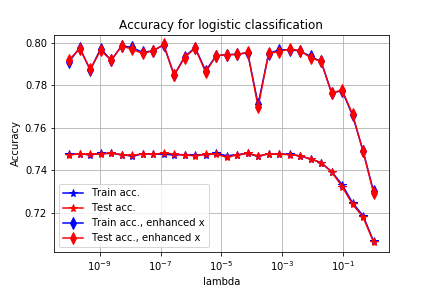
\includegraphics[width=0.45\textwidth]{accuracy_logistic.png}
	\caption{10000 iterations, $\gamma$ = 0.001}
\end{figure}

\begin{figure}[H]
	\centering
	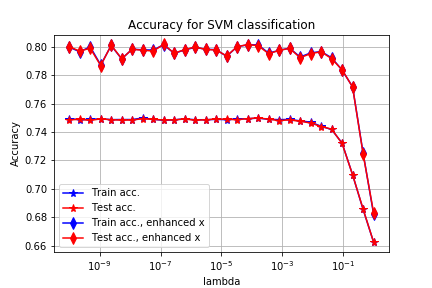
\includegraphics[width=0.45\textwidth]{accuracy_SVM.png}
	\caption{10000 iterations, $\gamma$ = 0.001}
\end{figure}

%%% TODO: same for SVM

%%% Comment on: overfit or underfit
\section*{Conclusion}
We presented a classifier based on support vector machines and using polynomial basis expansions which outperformed all other classifiers examined in the scope of the project in terms of accuracy. However, only classifiers based SVMs and logistic regression were assessed, a better performance may be achieved using other, more sophisticated classification models such as kernel SVMs, random forest or neural networks. 
\par
A downside of support vector machines is that they only output the class, but not a class probability. This makes it impossible to apply a more stringent cutoff for the detection of Higgs bosons in order to reduce the type I error. 
\par
Moreover, we assessed variable importance using forward-greedy best subset selection. (WAS GSEHT ME??? ) 
%%% Bibliography
\bibliographystyle{IEEEtran}
\bibliography{literature-project1}

\end{document}